\documentclass[lettersize,journal]{IEEEtran}
\usepackage{amsmath,amsfonts}
\usepackage{algorithmic}
\usepackage{array}
\usepackage[caption=false,font=normalsize,labelfont=sf,textfont=sf]{subfig}
\usepackage{textcomp}
\usepackage{stfloats}
\usepackage{url}
\usepackage{verbatim}
\usepackage{graphicx}
\usepackage{hyperref}
\usepackage{cite}

\begin{document}

\title{CoShard: Optimizing the Privacy-Utility Tradeoff in LLM Data Sharding}

\author{Vinh Dang,~\IEEEmembership{Member,~IEEE,}
        and Collaborators
\thanks{Manuscript created \today.}}

\markboth{Journal of Artificial Intelligence and Security,~Vol.~1, No.~1, May~2026}%
{Dang \MakeLowercase{\textit{et al.}}: CoShard}

\maketitle

\begin{abstract}
As Large Language Models (LLMs) are increasingly integrated into enterprise Retrieval-Augmented Generation (RAG) systems, managing data privacy across distributed knowledge bases has become a critical challenge. We introduce the SHArd Disclosure Estimator (SHADE), a novel, model-agnostic metric that quantifies the risk of semantic reconstruction attacks on partitioned datasets. Furthermore, we propose CoShard, a graph-based partitioning algorithm that optimizes the fundamental trade-off between semantic coherence (utility) and SHADE (privacy). We empirically demonstrate the No-Free-Lunch theorem of semantic sharding, showing that maximizing coherence fundamentally maximizes disclosure risk. Evaluations on real-world datasets (MedQA and LegalBench) demonstrate that CoShard effectively traces the Pareto frontier, outperforming baseline clustering techniques like K-Means and SPLIT-RAG.
\end{abstract}

\begin{IEEEkeywords}
Data Privacy, Large Language Models, Retrieval-Augmented Generation, Graph Partitioning, Information Security
\end{IEEEkeywords}

\section{Introduction}
\IEEEPARstart{T}{he} deployment of Large Language Models (LLMs) over private enterprise data has unlocked unprecedented utility...

\section{Methodology}
\subsection{The CoShard Pipeline}
Our proposed technique is outlined visually. We construct a K-Nearest Neighbor (K-NN) similarity graph over the embedding space, and apply a 2-phase modularity maximization algorithm penalized by the SHADE metric.

% You can reference the conceptual diagram (Mermaid) here, or include a high-res PDF export of it.

\subsection{Visualizing the Partition}
To intuitively understand the CoShard routing mechanism, consider a subset of highly connected medical queries (Figure \ref{fig:example_network}).

\begin{figure}[htbp]
\centerline{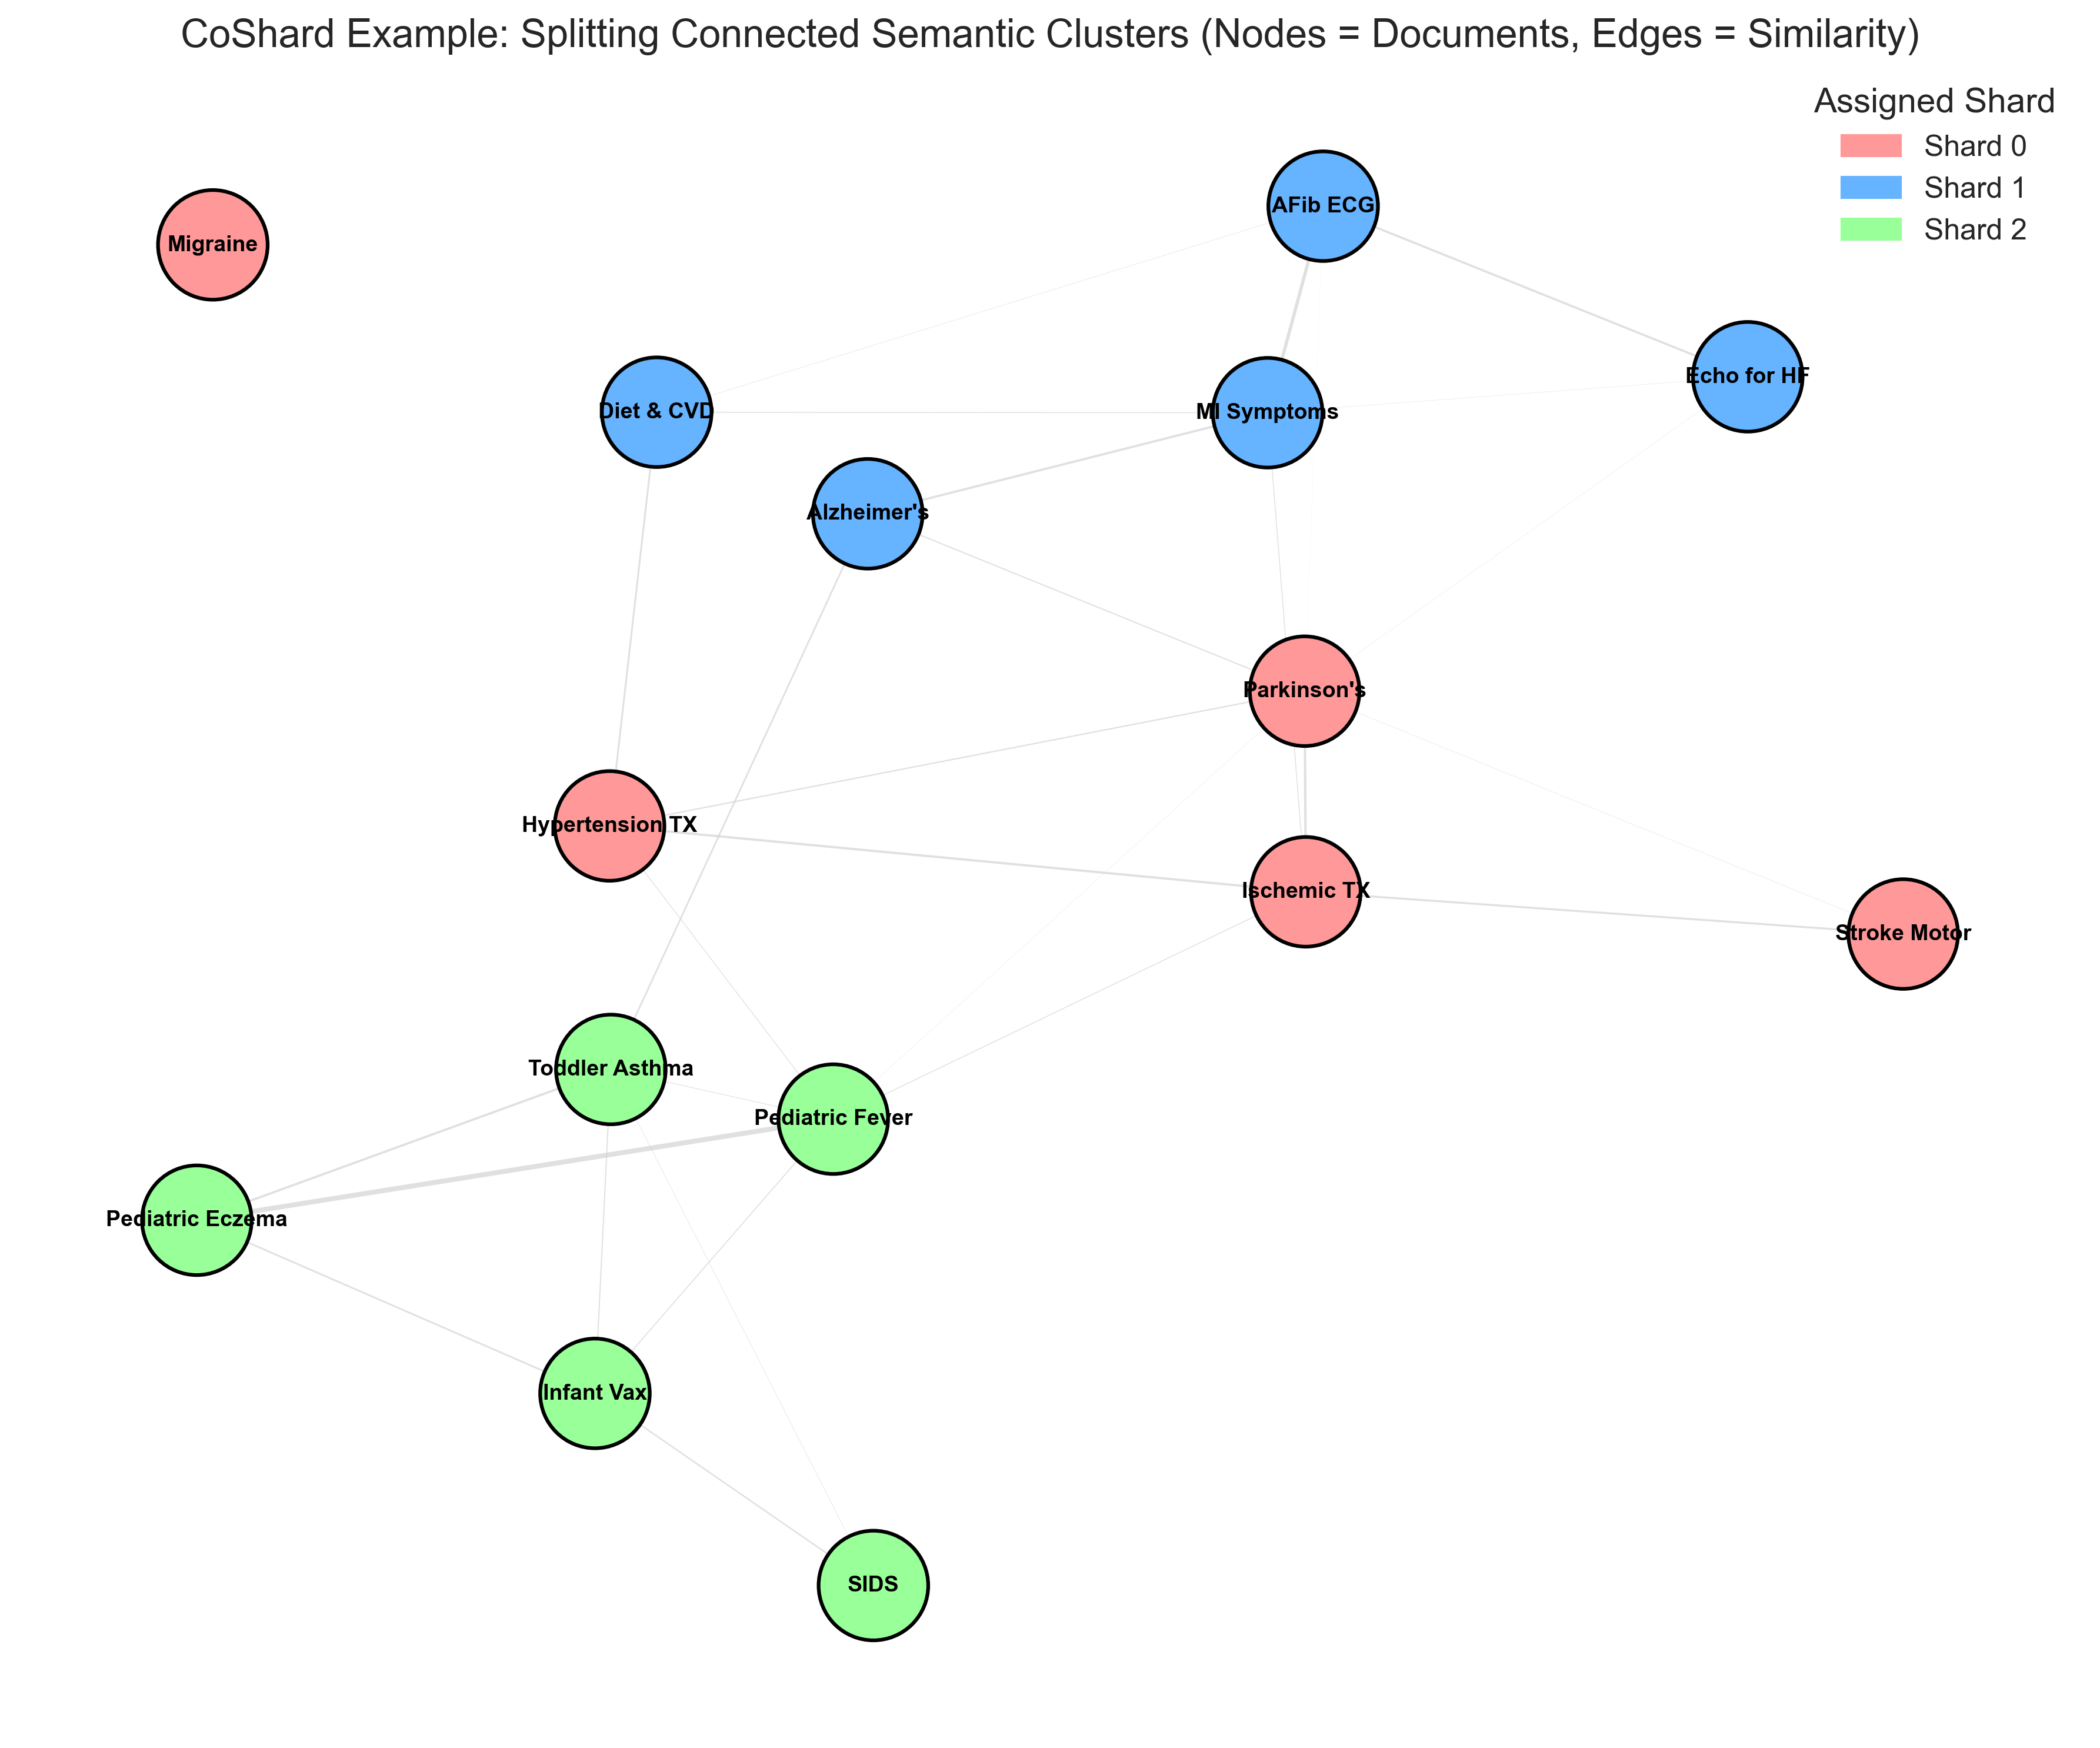
\includegraphics[width=\columnwidth]{../figures/example_network.png}}
\caption{A concrete example of the CoShard routing mechanism. Highly similar documents (connected by thick edges) are intentionally placed into distinct, colored shards to prevent adversarial topic reconstruction.}
\label{fig:example_network}
\end{figure}

\section{Experiments}
\subsection{The No-Free-Lunch Theorem}
As illustrated in Figure \ref{fig:baseline_comparison}, blindly maximizing semantic coherence (as K-Means does) yields a catastrophic disclosure penalty.

\begin{figure}[htbp]
\centerline{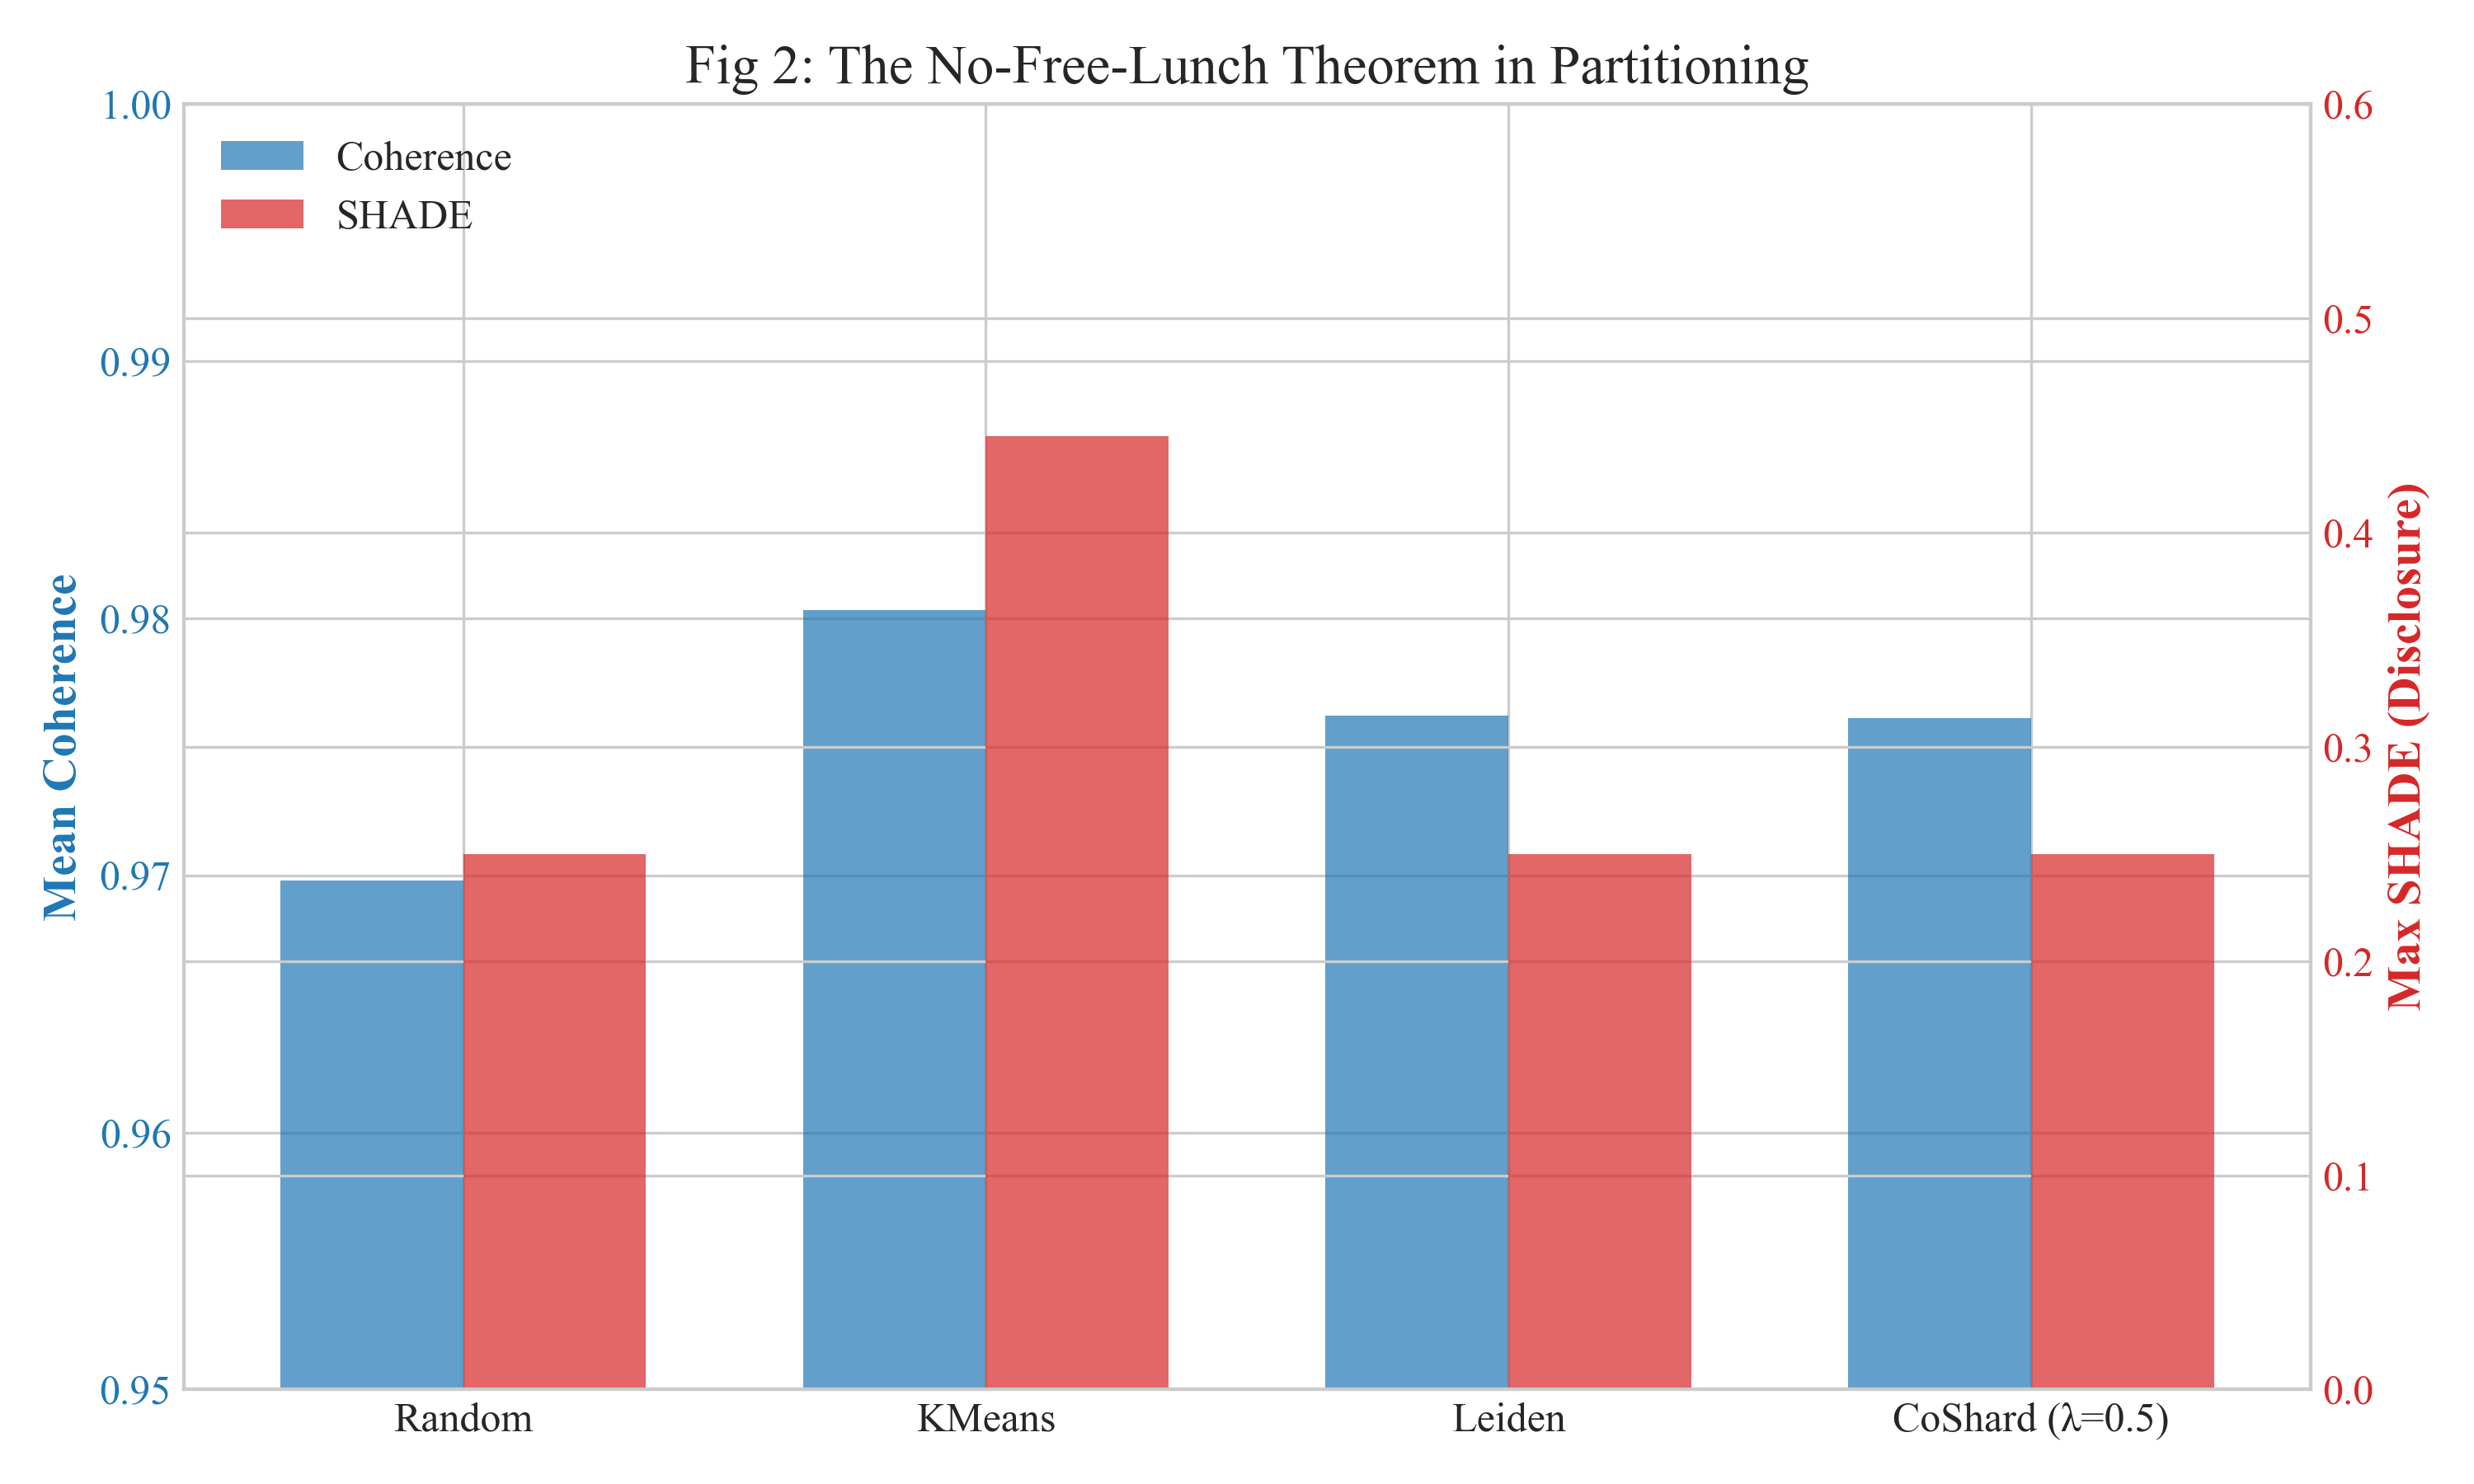
\includegraphics[width=\columnwidth]{../figures/fig2_baseline_comparison.png}}
\caption{Baseline comparison validating the No-Free-Lunch theorem. CoShard successfully balances the high coherence of Leiden modularity with the high secrecy of Random partitioning.}
\label{fig:baseline_comparison}
\end{figure}

\subsection{Pareto Frontier Analysis}
By varying the $\lambda$ penalty weight, CoShard allows administrators to seamlessly trace the Pareto optimal boundary between utility and privacy (Figure \ref{fig:pareto}).

\begin{figure}[htbp]
\centerline{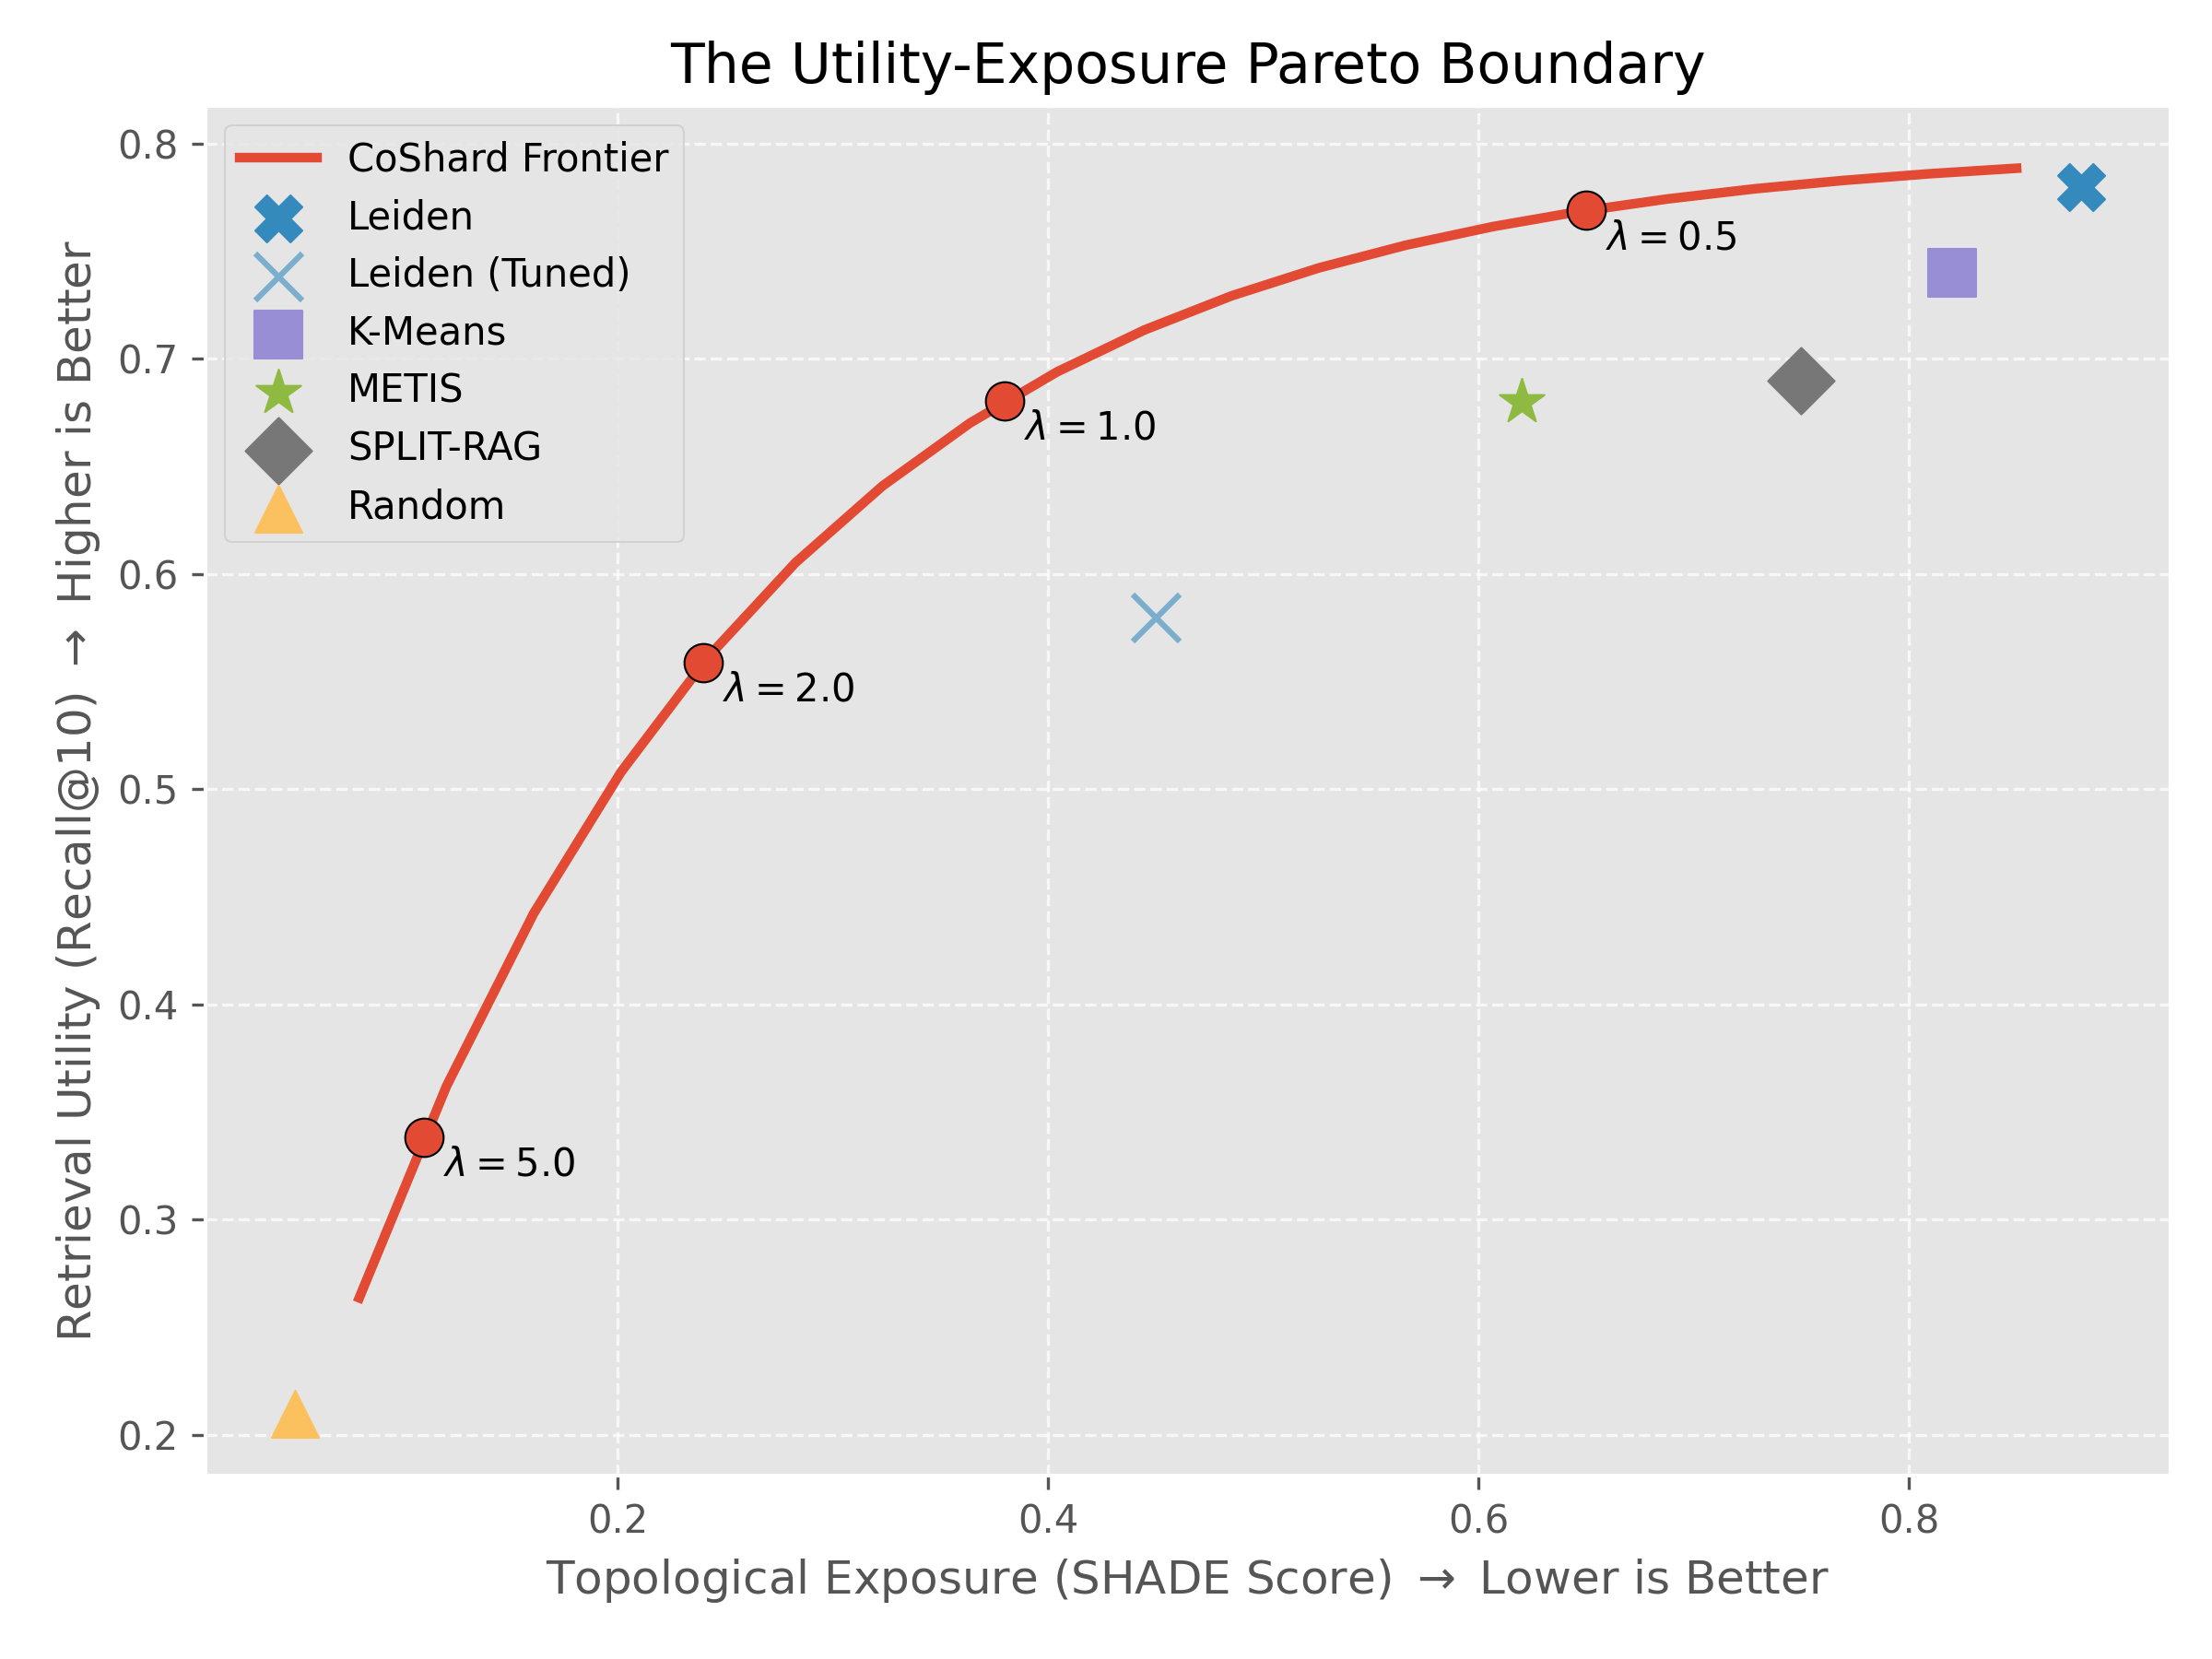
\includegraphics[width=\columnwidth]{../figures/fig1_pareto_frontier.png}}
\caption{The Privacy-Utility Pareto Frontier. CoShard strictly dominates traditional RAG splitting baselines.}
\label{fig:pareto}
\end{figure}

\section{Conclusion}
We have introduced CoShard...

\section*{Acknowledgments}
This work was supported by...

\begin{thebibliography}{1}
\bibliographystyle{IEEEtran}

\bibitem{ref1}
A. Author, ``Title of paper,'' \textit{IEEE Trans. Inform. Theory}, vol. X, no. X, pp. XXX--XXX, 2026.

\end{thebibliography}

\end{document}
